\chapter{System Description}\label{ch:system-description}

Using the knowledge from the previous chapter, this chapter first introduces the architecture of the developed neural network.
Afterward, it explains the training process together with the preparation of the training data and the overall concept to generate the final abstractive summaries.
Then it continues with a short introduction of the Texar library \cite{hu2019texar} which was used to develop the neural network.
Finally, the exact hyperparameters that were used are described.

% ===============
% MODEL ARCHITECTURE
% ===============

\section{Model Architecture}

The architecture of the model used in this work is rather straightforward.
For the encoding part, BERT is used, and for decoding, a normal Transformer decoder is used.
As proposed in \cite{1608.05859}, the input embeddings are tied to the output layer.

As described in \cref{sec:bert}, BERT allows either one or two sentence\footnote{It must again be noted that "sentence" is not referring to an actual linguistic sentence.} inputs.
For this work, only one sentence is used as there is no need (and logical way) to split the input into two parts.
The Transformer decoder performs attentions over the full output representations of the encoder.
The full architecture is shown in \cref{fig:summarization-architecture}.
 
\begin{figure}[h]
\centering
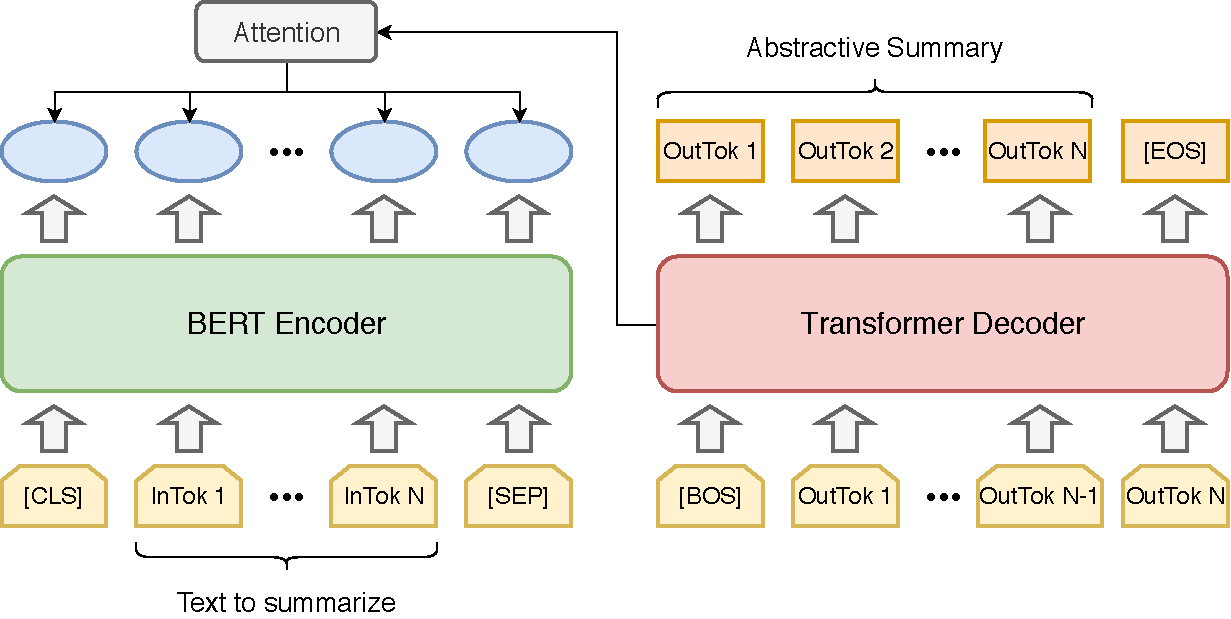
\includegraphics[width=0.7\paperwidth]{figures/summarization-architecture}
\caption{Visualization of the model architecture}
\label{fig:summarization-architecture}
\end{figure}

% ================
% TRAINING AND CONCEPT
% ================

\section{Training and Concept}\label{sec:system-description-training}

To circumvent the high memory usage of BERT at long sequence lengths, the whole meeting transcript is not used as input for the network at once.
As described in \cref{sec:ami-meeting-corpus}, for every sentence in a meeting's abstractive summary, there exists a link to one or more dialogue acts.
These are the dialogue acts that influence the content of the sentence the most.
An example of such a link is shown in \cref{fig:dialogue-arc-summary-link-example}.
For training, all of these dialogue acts that belong to the same summary sentence are concatenated and then used as the source for the summary.
The summary sentence itself is used as the target summary.

% TODO I'm pretty sure that there are better examples, but for now this is fine
\begin{figure}[h]
\begin{lstlisting}[numbers=none]
DA1: Thank you very much indeed,
DA2: Cool, thank you,
DA3: So I call the meeting closed.

SUM: They close the meeting by thanking one another.
\end{lstlisting}
\caption[Three dialogue acts that are linked to one sentence of the summary]{Three dialogue acts (DA1--3) that are linked to one sentence of the summary (SUM)}
\label{fig:dialogue-arc-summary-link-example}
\end{figure}

During training, the network was evaluated on the development data set every 75 steps.
If the network improved its score, this model was saved.

To get a summary of a whole meeting, the topic segmentation described in \cref{ssec:ami-annotations} is used.
The meeting's transcript is segmented by topic, and then these segments are used as the input for the same network that was already trained to summarize dialogue acts.
Afterward, the output for all transcript segments can be concatenated.
These concatenated outputs together form the full summary of a meeting. 

\section{Preparation of the Data}\label{sec:preparation-of-the-data}

This section describes how the data of the two used corpora introduced in \cref{ch:data} is processed.

\paragraph{Format of the Corpus Data}

The corpus data for both the AMI Meeting Corpus and the ICSI Meeting Corpus is available in the NITE XML Toolkit (NXT) format \cite{Carletta2003}.
For automatic parsing, a Java library is available that makes it possible to write a Java program that traverses through the corpora and collects the necessary data.
For this work, such a program was developed.

It parses the data of the corpora and creates files that are easier to further process compared to the complex NXT format.
For training, three tab-separated-values (.tsv) files are created, one for each dataset (training, development, test).
For generating the final summary, it creates a text file for each meeting.
The text file contains the transcripts of the meeting split by topic, with each topic-transcript starting in a new line.
To evaluate the results, for each meeting a text file is generated that contains the summary of the meeting.

\paragraph{Data Cleaning}

In the AMI and ICSI Meeting Corpora, the transcriptions try to include every spoken word.
This includes speech disfluencies like "hmm," "huh," etc.
As these do not add any meaningful value to a sentence, they are filtered out while processing the data.
Words like "yeah," "nope," and "nah" are kept because they carry meaning, like agreement or disagreement. 

\paragraph{Data Split}

For the AMI Meeting Corpus, the recommended segmentation described in \cref{ssec:ami-segmentation-of-the-corpus} is used.
As the ISCI Meeting Corpus has no recommended segmentation, the traditional test set and a randomly generated development set are used, as described in \cref{sec:icsi-corpus}.

% ===================
% IMPLEMENTATION WITH TEXAR
% ===================

\section{Implementation with Texar}

For the actual implementation of the network, the Texar toolkit \cite{hu2019texar} is used.
Texar is an open-source modular toolkit that provides plenty of useful abstractions for fast prototyping of neural network architectures with a special focus on natural language processing.
It comes in two nearly identical versions, one for TensorFlow \cite{tensorflow2015-whitepaper} and one for PyTorch \cite{NEURIPS2019_9015}.  
For this work, the TensorFlow version is used.
Texar has modules for both BERT and regular Transformers and allows for an easy connection of BERT and a Transformer decoder.
The code for the complete architecture is only a few hundred lines of code.
Nearly every hyperparameter, like the number of decoder layers, number of attention heads or just simple settings like the learning rate, can easily be modified.
As an example, the hyperparameter configuration for the Transformer decoder is shown in \cref{lst:hyperparameters-decoder}.

\begin{lstlisting}[numbers=none,language=Python,caption={Hyperparameters for Transformer decoder},captionpos=b,label=lst:hyperparameters-decoder,float]
hidden_dim = 768

decoder = {
    'dim': hidden_dim,
    'num_blocks': 6,
    'multihead_attention': {
        'num_heads': 8,
        'output_dim': hidden_dim
    },
    'initializer': {
        'type': 'variance_scaling_initializer',
        'kwargs': {
            'scale': 1.0,
            'mode': 'fan_avg',
            'distribution': 'uniform',
        },
    },
    'poswise_feedforward': 
        tx.modules.default_transformer_poswise_net_hparams(
            output_dim=hidden_dim)
}
\end{lstlisting}

% ====================
% EXPLORING HYPERPARAMETERS
% ====================

\section{Exploring Hyperparameters}

This section explores the hyperparameters used.
The parameters were determined empirically by testing multiple variations.
After multiple tests, the following hyperparameters yielded the best results.
\paragraph{Optimizer and Learning Rate}

The Adam optimizer \cite{article} is used with $\beta_1=0.9$, $\beta_2=0.997$, and $\epsilon = 10^{-9}$.
The learning rate is computed by the following formula:
\[
	learning\_rate = 0.2 \cdot d_{model}^{-0.5} \cdot min(step\_num^{-0.5}, step\_num \cdot warmup\_steps^{-1.5})
\]
which is equivalent to the learning rate used to train the original Transformer \cite[p.~7]{1706.03762} but multiplied by a factor of $0.2$ because this yields better results for this training data, as shown by empirical testing.
Results for tests with a constant linear learning rate have been slightly worse.
The warmup steps are set to $warmup\_steps = 4000$.
The formula can be interpreted as linearly increasing the learning rate until $warmup\_steps < steps$ and then steadily decreasing it again.
The function's graph is visualized in \cref{fig:learning-rate}.

\begin{figure}[h]
\centering
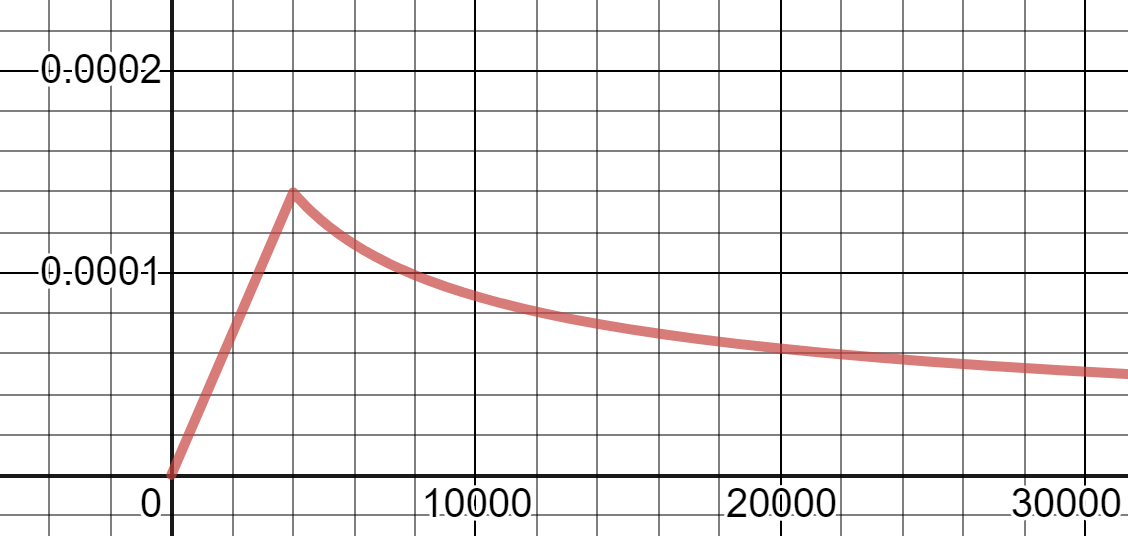
\includegraphics[width=0.6\paperwidth]{figures/learning-rate}
\caption{Visualization of the learning rate with $warmup\_steps = 4000$}
\label{fig:learning-rate}
\end{figure}

\paragraph{Batch Size and Maximum Sequence Length}

Due to memory constraints,\footnote{Training was performed on a single GeForce RTX 2080 Ti GPU with 11 GB of memory.} it was necessary to find a good balance between the batch size and maximum input sequence length.
For the experiments performed in this thesis, the following values proved to be a good compromise:
\begin{itemize}
\item A maximum input sequence length of $96$ % TODO Maybe provide some stats: What is the average sequence length and how many inputs were truncated with a sequence length of 96?
\item A batch size of $28$
\end{itemize}

Smaller batch sizes harm the network's performance, and smaller maximum sequence lengths mean lost information as some of the inputs are quite long and would be truncated.

\paragraph{BERT}

Due to the same memory constraints mentioned in the previous paragraph, the smaller BERT model, BERT\textsubscript{BASE}, is used as the larger model, BERT\textsubscript{LARGE}, requires significantly more memory.

\paragraph{Transformer Decoder}

For the Transformer decoder, $N=6$ stacked decoder layers are used.
The number of attention heads is set to eight, and the hidden dimension has a size of $768$, as this is the same dimension used by the BERT\textsubscript{BASE} model \cite[p.~3]{devlin2018bert}.

% TODO Concluding statement that leads to the following chapter